\documentclass[a4paper,12pt]{report}
\usepackage[utf8]{inputenc}
\usepackage[francais]{babel}
\usepackage{fancyhdr}
\usepackage{graphicx}
\usepackage{tikz}
\usetikzlibrary{calc}
\usepackage{listings}
\usepackage{xcolor}
\definecolor{grey}{rgb}{0.9,0.9,0.9}
\usepackage{titlesec}
\usepackage{verbatim}
\usepackage{listings}
\usepackage{textcomp}
\usepackage{hyperref}
\usepackage{amssymb}
\usepackage{amsmath}
\usepackage{longtable}
\usepackage{colortbl}
\usepackage{float}
\usepackage{caption}
\usepackage{subfig}
\usepackage{color}
\usepackage{colortbl}
\frenchbsetup{StandardLists=true}
\newcommand{\marge}{18mm}
\usepackage[left=\marge,right=\marge,top=\marge,bottom=\marge]{geometry}
\pagestyle{fancy}
\setlength{\headheight}{14pt}
\renewcommand{\headrulewidth}{1pt}
\linespread{1}
\setlength{\columnseprule}{0.2pt}
\title{TP9 TI : Detection de contours}
\author{DOUAILLE Erwan et NAIT ABDELAZIZ Yanis}

\lstset{ %
  language=java,                  % the language of the code
  basicstyle=\footnotesize,       % the size of the fonts that are used for the code
  numbers=left,                   % where to put the line-numbers
  numberstyle=\tiny\color{gray},  % the style that is used for the line-numbers
  stepnumber=1,                   % the step between two line-numbers. If it's 1, each line
                                  % will be numbered
  numbersep=5pt,                  % how far the line-numbers are from the code
  backgroundcolor=\color{white},  % choose the background color. You must add \usepackage{color}
  showspaces=false,               % show spaces adding particular underscores
  showstringspaces=false,         % underline spaces within strings
  showtabs=false,                 % show tabs within strings adding particular underscores
  frame=single,                   % adds a frame around the code
  rulecolor=\color{black},        % if not set, the frame-color may be changed on line-breaks within not-black text (e.g. commens (green here))
  tabsize=2,                      % sets default tabsize to 2 spaces
  captionpos=b,                   % sets the caption-position to bottom
  breaklines=true,                % sets automatic line breaking
  breakatwhitespace=false,        % sets if automatic breaks should only happen at whitespace
  title=\lstname,                 % show the filename of files included with \lstinputlisting;
                                  % also try caption instead of title
  keywordstyle=\color{blue},      % keyword style
  commentstyle=\color{green},   % comment style
  stringstyle=\color{magenta},      % string literal style
  escapeinside={\%*}{*)},         % if you want to add a comment within your code
  morekeywords={*,...}            % if you want to add more keywords to the set
} 

\begin{document}
\maketitle
%%%%%%%%%%%%%%%%%%%%%%%%%%%%%%%%%%%%%Introduction%%%%%%%%%%%%%%%%%%%%%%%%%%%%%%%%%%%%%%%%%%%%%
\section*{Introduction}
Dans ce tp nous allons voir comment procéder à une détection de contours par approche du premier ordre notamment par le calcul de la norme du gradient ainsi que différentes techniques de seuillage.

%%%%%%%%%%%%%%%%%%%%%%%%%%%%%%%%%%%%%%%%%%%%%%%%%%%%%%%%%%%%%%%%%%%%%%%%%%%%%%%%%%%%%%%%%%%%%%
\section*{Seuillage de la norme du gradient}
\subsection*{Q2- Norme du gradient}
\begin{lstlisting}
// Calculs pour chaque pixel
for (j=0; j<h; j++) {
	for (i=0; i<w;i++) {
		selectImage(filenameGradX);
		px = getPixel(i,j);
		selectImage(filenameGradY);
		py = getPixel(i,j);
		norme = sqrt(px*px+py*py);

		selectImage(nouvelle_Image);
		setPixel(i,j, norme);	
	}
}
setBatchMode("exit and display");
\end{lstlisting}
Le code ci-dessus permet de calculer la norme du gradient et ainsi on obtient l'image suivante:
\begin{figure}[!ht]
	\center
	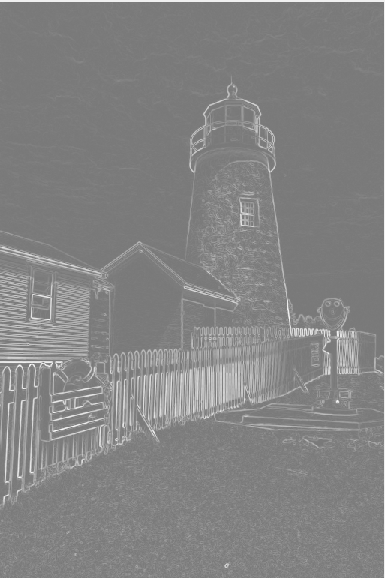
\includegraphics[scale=0.3]{./imageResultats/gradient_q2.png}
\end{figure}
\subsection*{Q3-Analyse}
Lorsqu'on affiche l'histogramme de l'image correspondant à la norme du gradient , on obtient comme valeur minimale 0 et comme valeur maximale 904. Ceci est du au fait que l'image est une image codée sur 32 bits et au calcul de la valeur des pixels : sqrt(px*px+py*py).
\subsection*{Q4-Comparaison}
Afin d'obtenir une image similaire à celle calculée par imagej, on doit changer le contraste de l'image pour obtenir des valeurs comprises entre 0 et 255 et changer le type de l'image en le mettant à 8 bits.
\begin{figure}[!ht]
	\begin{center}
		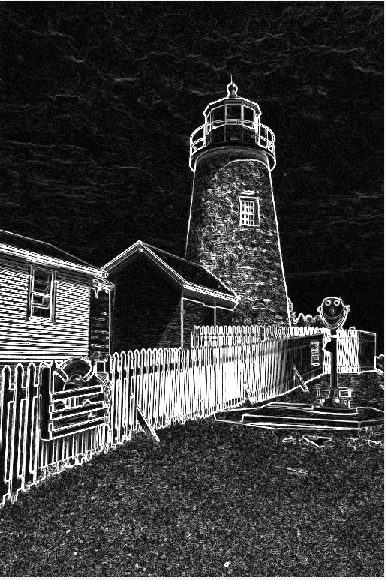
\includegraphics[scale=0.4]{./imageResultats/norme_gradient_q4.png}
		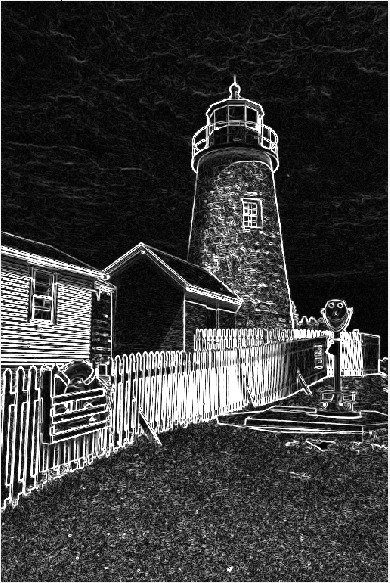
\includegraphics[scale=0.4]{./imageResultats/gradient_imagej.png}
	\end{center}
L'image de gauche est l'image pour laquelle nous avons modifié le contraste et l'image de droite est l'image calculée par imagej. Maintenant, lorsqu'on soustrait les deux images, on obtient une image dont tous les pixels sont égaux à 0, donc les deux images sont identiques.
\end{figure}
\newpage
\subsection*{Q5-Seuillage de la norme du gradient précédemment calculé}
Le seuil de la norme du gradient estimé est égal à 120. Il est difficile de trouver un seuil global pour l'image qui mette en évidence les pixels contours de manière satisfaisante. En effet si on prend un seuil trop bas , on aura beaucoup de bruit et si on prend un seuil trop haut on n'aura pas tous les pixels correspondant aux contours. Ainsi avec ce seuil , on obtient l'image suivante:
\begin{figure}[!ht]
	\center
	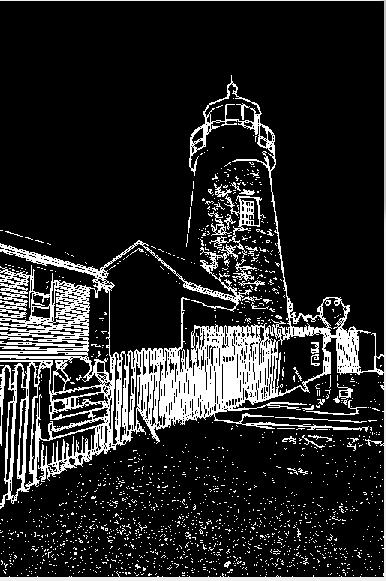
\includegraphics[scale=0.4]{./imageResultats/seuillage_q5.png}
\end{figure}
\subsection*{Q6-Seuillage semi automatique}
En prenant les 20\% des pixels de la norme du gradient , on obtient un seuil d'une valeur de 97. En utilisant la valeur de ce seuil avec les contours en noir, on obtient une image ou les contours sont plus satisfaisant que les images précedentes.
\begin{figure}[!ht]
	\center
	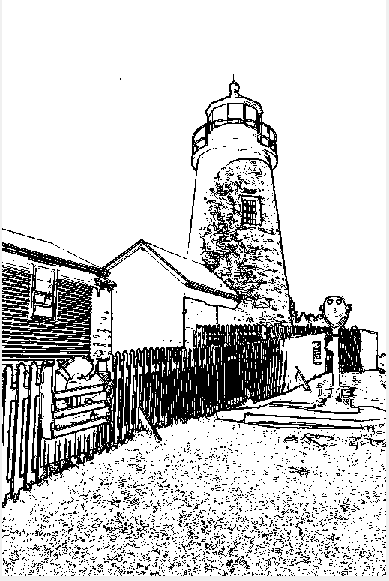
\includegraphics[scale=0.4]{./imageResultats/norme_gradient_q6.png}
\end{figure}
\section*{Détection des maxima locaux}
Dans cette partie, nous allons apporter une modification à ce que nous avons fait précédemment ou on éliminera les non-maxima locaux; ce qui permettra d'obtenir des résultats plus satisfaisants.
\subsection*{Q1-Direction du gradient}
L'image correspondante à la direction du gradient ne permet pas de bien distinguer les contours.
\begin{figure}[!ht]
	\center
	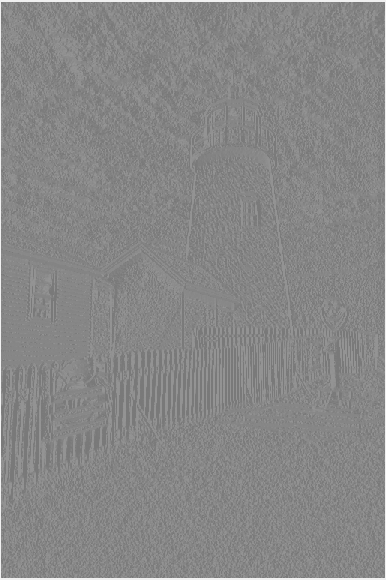
\includegraphics[scale=0.4]{./imageResultats/partie2_q1.png}
\end{figure}
\subsection*{Q2-Analyse de l'image}
Après observation des valeurs avec  l'outil \emph{Pixel Inspector}  on observe des valeurs de pixels comprises entre 170 et 180 degrés.
\subsection*{Q3-Macro}
Le macro  permettant d'éliminer les non-maxima locaux de la norme du gradient nous permet d'obtenir l'image suivante :
\begin{figure}[!ht]
	\center
	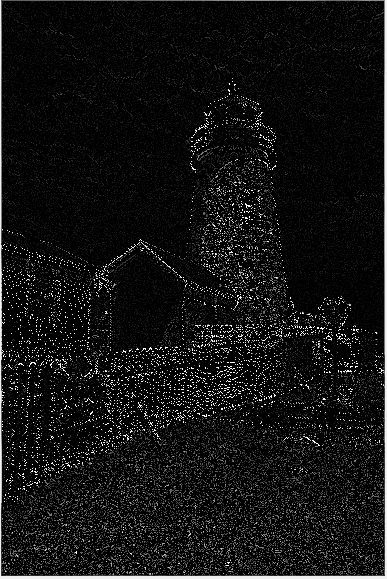
\includegraphics[scale=0.4]{./imageResultats/maxima.png}
\end{figure}
\subsection*{Q4- Comparaison}
Le résultat n'est pas très satisfaisant, il doit sûrement y avoir une erreur dans la macro
\section*{Conclusion}
Dans ce tp, nous avons réussi à déterminer les contours d'une image en utilisant une approche du premier ordre. On peut retenir que si on n'utilise seule la norme du gradient ne suffit pas. On doit en plus de cela seuiller la norme du gradient. Pour cela , nous avons éliminé les non-maxima locaux.
\section*{Annexe}
\begin{lstlisting}
requires("1.41i");	// requis par substring(string, index)
setBatchMode(true);

sourceImage = getImageID();
filename = getTitle();

/********** Recuperation des infos de l'image originale **************/
// recuperation de la taille de l'image
w = getWidth();
h = getHeight();

/************************* Creation title ***************************/
extension = "";
if (lastIndexOf(filename, ".") > 0) {
    extension = substring(filename, lastIndexOf(filename, "."));
    filename = substring(filename, 0, lastIndexOf(filename, "."));
}
filenameGradX = filename+"_grad_x"+extension;
filenameGradY = filename+"_grad_y"+extension;
/*******************Convultion selon l'axe X **********************/
run("Duplicate...", "title="+filenameGradX);
run("32-bit");
run("Convolve...","text1=[-1 0 1 \n -2 0 2 \n -1 0 1 \n] normalize");

convolutionX = getImageID();
/****************************************************************/
selectImage(sourceImage);
/*******************Convultion selon l'axe Y**********************/
run("Duplicate...", "title="+filenameGradY);
run("32-bit");
run("Convolve...","text1=[-1 -2 -1 \n 0 0 0 \n 1 2 1 \n] normalize");
convolutionY = getImageID();
/***************************************************************/
resultat = filename+"ResultatNorme";
run("Duplicate...", "title=resultat norme");
nouvelle_Image = getImageID();

resultat1 = filename+"ResultatDirection";
run("Duplicate...", "title=resultat direction");
nouvelle_Image_Direction = getImageID();

// Calculs pour chaque pixel
for (j=0; j<h; j++) {
	for (i=0; i<w;i++) {
		selectImage(convolutionX);
		px = getPixel(i,j);
		selectImage(convolutionY);
		py = getPixel(i,j);
		norme = sqrt(px*px+py*py);

		directionGradient = abs(atan2(py,px)*180/PI);

		selectImage(nouvelle_Image);
		setPixel(i,j, norme);
		
		selectImage(nouvelle_Image_Direction);
		setPixel(i,j, directionGradient);
		
	}
}
selectImage(sourceImage);
run("Duplicate...", "title=maxima");
maxima=getImageID();
for(j=1 ;j<h-1 ; j++){
	for(i=1 ; i<w-1 ; i++){
		x1=i;
		x2=i;
		y1=j;
		y2=j;
		selectImage(nouvelle_Image_Direction);
		val = round(getPixel(i,j)/45)*45;
		selectImage(nouvelle_Image);
			if(val==180 || val==-180){
				y1=j-1;
				y2=j+1;
			}
			if(val==135 || val==-45){
				x1=i+1;
				x2=i-1;
				y1=j-1;
				y2=j+1;
			}
			if(val==90 || val==-90){
				x1=i-1;
				x2=i+1;			}
			if(val==45 || val==-135){
				x1=i+1;
				x2=i-1;
				y1=j+1;
				y2=j-1;
			}
			if(val==0){
				y1=j-1;
				y2=j+1;
			}
			
			p1=getPixel(x1,y1);
			p2=getPixel(x2,y2);
			p=getPixel(i,j);
			if(p<p1 || p<p2)
				p=0;
			selectImage(maxima);
			setPixel(i,j,p);
	}
}
setBatchMode("exit and display");
\end{lstlisting}
\end{document}
